\documentclass{article}
\usepackage{morris}
\usepackage{diagbox}
\usepackage{centernot}
\usepackage{tikz}

\newcommand{\indep}{\mathrel{\text{\scalebox{1.07}{$\perp\mkern-10mu\perp$}}}}
\newcommand{\nindep}{\centernot{\indep}}

\renewcommand{\thesection}{Problem \arabic{section}.}
\renewcommand{\thesubsection}{\arabic{subsection}.}
\renewcommand{\thesubsubsection}{\alph{subsubsection})}

\title{Machine Learning 2 --- Homework 2}
\author{%
  Maurice Frank\\
  11650656\\
  \href{mailto:maurice.frank@posteo.de}{maurice.frank@posteo.de}
}

\begin{document}
\maketitle

\section{}
\subsection{}
We have the discrete random variables \(X, Y, Z\).
Mutual information than is:
\begin{align*}
    I(X;Y)
    &= \KL(p(x,y)||p(x)p(y))\\
    &= \mathcal{H}(X) - \mathcal{H}(X|Y)
\end{align*}

The conditional mutual information is:
\begin{align*}
    I(X;Y|Z)
    &= \E_{p(z)}[\KL(p(x,y|z)||p(x|y)p(y|z))]\\
    &= \mathcal{H}(X|Z) - \mathcal{H}(X|Y,Z)
\end{align*}

We see that the conditional mutual information measures the expected mutual information between \(X\) and \(Y\) given \(Z\).

\subsection{}
We have \(x,y,z\∈\{0,1\}\) with \(p(x,y,z)\).
First we will write down \(p(x,y)\) (see Table~\ref{tab:margin_z}), \(p(x)\) and \(p(y)\) (see Table~\ref{tab:margin_y_x}).

\begin{table}
    \centering
    \begin{tabular}{ccc}
        X & Y & p(x,y)\\\toprule
        0 & 0 & 0.336\\
        0 & 1 & 0.264\\
        1 & 0 & 0.256\\
        1 & 1 & 0.144
    \end{tabular}
    \caption{Marginalizing Z.}
    \label{tab:margin_z}
\end{table}

\begin{table}
    \centering
    \begin{tabular}{c|cc|c}
        \diagbox{X}{Y} & 0 & 1 & p(x)\\\hline
        0 & 0.336 & 0.264 & 0.6\\
        1 & 0.256 & 0.144 & 0.4\\\hline
        p(y) & 0.592 & 0.408 & 1
    \end{tabular}
    \caption{Marginalizing X and Y.}
    \label{tab:margin_y_x}
\end{table}

\begin{align*}
    I(X;Y)
    &= \KL(p(x,y)||p(x)p(y))\\
    &= -\Σ_{x,y} p(x,y)\ln{(\÷{p(x)p(y)}{p(x,y)})}\\
    &= 3.197\·10^{-3}\\
    &> 0
\end{align*}

As the mutual information between \(X\) and \(Y\) is bigger than zero (it is symmetric!) we showed that having knowledge about one of the values we gain knowledge about the possible distribution of values of the second variable.
We see this with \(I(X;Y) = \mathcal{H}(X) - \mathcal{H}(X|Y) > 0 \⇒ \mathcal{H}(X|Y) < \mathcal{H}(X)\), the entropy of one given the other is lower than without this conditional information.

\subsection{}

\begin{table}
    \centering
    \begin{tabular}{cccc}
        \diagbox{x}{y} & 0 & 1 & p(x|z=0)\\\hline
        0 & 0.4 & 0.1 & 0.5\\
        1 & 0.4 & 0.1 & 0.5\\
        p(y|z=0) & 0.8 & 0.2 & 1.0
    \end{tabular}
    \caption{p(x,y|z=0) and p(x|z=0), p(y|z=0)}
    \label{tab:xyz0}
\end{table}
\begin{table}
    \centering
    \begin{tabular}{cccc}
        \diagbox{x}{y} & 0 & 1 & p(x|z=1)\\\hline
        0 & 0.277 & 0.415 & 0.692\\
        1 & 0.123 & 0.185 & 0.308\\
        p(y|z=1) & 0.4 & 0.6 & 1.0
    \end{tabular}
    \caption{p(x,y|z=1) and p(x|z=1), p(y|z=1)}
    \label{tab:xyz1}
\end{table}

See Table~\ref{tab:xyz0} and Table~\ref{tab:xyz1} for intermediate calculation tables.

\begin{align*}
    I(X;Y|Z)
    &=\hspace{0.8em} p(z=0)\·\KL(p(x,y|z=0)||p(x|z=0)p(y|z=0))\\
    &\quad + p(z=1)\·\KL(p(x,y|z=1)||p(x|z=1)p(y|z=1))\\
    &= -\Σ_{z\∈ Z}p(Z=z)\·\Σ_{x,y}p(x,y|z)\·\log{(\÷{p(x|z)p(y|z)}{p(x,y|z)})}\\
    &= -(0.48\·0 + 0.52\·0)\\
    &= 0
\end{align*}

That now the conditional mutual information is zero tells us that given that we know about the value of \(Z\) than having information about \(X\) or \(Y\) will not tell us anything about the respective third variable.
\(I(X;Y|Z) = 0\⇒ \mathcal{H}(X|Z) = \mathcal{H}(X|Y,Z) \wedge \mathcal{H}(Y|Z) = \mathcal{H}(Y|X,Z)\).

\subsection{}
For the Computation of \(p(x)\·p(z|x)\·p(y|z) = p(x,y,z)\) see Table~\ref{tab:lastxyz}.
The directed graph is show in Figure~\ref{fig:graph}.

\begin{table}
    \centering
    \begin{tabular}{lllllll}
        \(x\) & \(p(x)\) & \(z\) & \(p(z|x)\) & \(y\) & \(p(y|z)\) & \(p(x)\·p(z|x)\·p(y|z)\)\\\toprule
        0 & 0.6 & 0 & 0.4 & 0 & 0.8 & 0.192\\
        0 & 0.6 & 0 & 0.4 & 1 & 0.2 & 0.048\\
        0 & 0.6 & 1 & 0.6 & 0 & 0.4 & 0.144\\
        0 & 0.6 & 1 & 0.6 & 1 & 0.6 & 0.216\\
        1 & 0.4 & 0 & 0.6 & 0 & 0.8 & 0.192\\
        1 & 0.4 & 0 & 0.6 & 1 & 0.2 & 0.048\\
        1 & 0.4 & 1 & 0.4 & 0 & 0.4 & 0.064\\
        1 & 0.4 & 1 & 0.4 & 1 & 0.6 & 0.096\\
    \end{tabular}
    \caption{Computation of \(p(x)\·p(z|x)\·p(y|z)\)}
    \label{tab:lastxyz}
\end{table}

\begin{figure}
    \centering
    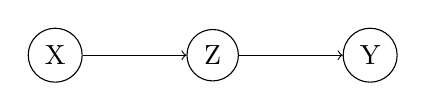
\begin{tikzpicture}
        \path (0,0) node[circle,draw](x) {X}
            (2,0) node[circle,draw](z) {Z}
            (4,0) node[circle,draw](y) {Y};
        \draw[->] (x) -- (z);
        \draw[->] (z) -- (y);
    \end{tikzpicture}
    \caption{The directed graph to the factorization \(p(x)p(z|x)p(y|z)\)}
    \label{fig:graph}
\end{figure}


\section{}
We strictly plot not the permutated directed graphs.
See Figures~\ref{tikz:bay_first} until \ref{tikz:bay_last}.

\begin{figure}
    \centering
    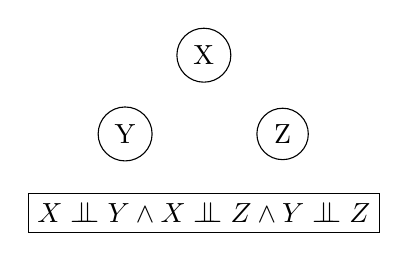
\begin{tikzpicture}
        \path (0,0) node[circle,draw](x) {X} (-1, -1) node[circle,draw](y) {Y} (1, -1) node[circle,draw](z) {Z};
        \draw (0, -2) node[draw] {$X\indep Y \wedge X\indep Z \wedge Y\indep Z$};
    \end{tikzpicture}
    \label{tikz:bay_first}
\end{figure}

\begin{figure}
    \centering
    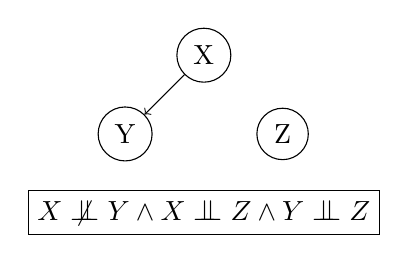
\begin{tikzpicture}
        \path (0,0) node[circle,draw](x) {X} (-1, -1) node[circle,draw](y) {Y} (1, -1) node[circle,draw](z) {Z};
        \draw[->] (x) -- (y);
        \draw (0, -2) node[draw] {$X\nindep Y \wedge X\indep Z \wedge Y\indep Z$};
    \end{tikzpicture}
\end{figure}

\begin{figure}
    \centering
    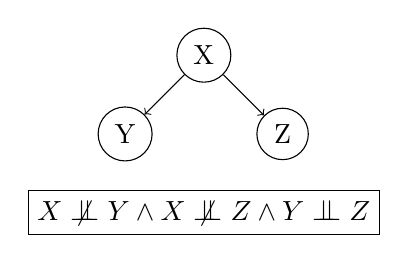
\begin{tikzpicture}
        \path (0,0) node[circle,draw](x) {X} (-1, -1) node[circle,draw](y) {Y} (1, -1) node[circle,draw](z) {Z};
        \draw[->] (x) -- (y);
        \draw[->] (x) -- (z);
        \draw (0, -2) node[draw] {$X\nindep Y \wedge X\nindep Z \wedge Y\indep Z$};
    \end{tikzpicture}
\end{figure}

\begin{figure}
    \centering
    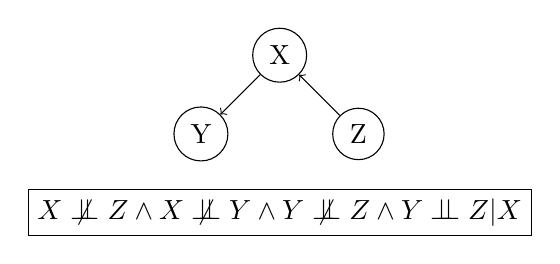
\begin{tikzpicture}
        \path (0,0) node[circle,draw](x) {X} (-1, -1) node[circle,draw](y) {Y} (1, -1) node[circle,draw](z) {Z};
        \draw[->] (x) -- (y);
        \draw[->] (z) -- (x);
        \draw (0, -2) node[draw] {$X\nindep Z \wedge X\nindep Y \wedge Y\nindep Z \wedge Y\indep Z|X$};
    \end{tikzpicture}
\end{figure}

\begin{figure}
    \centering
    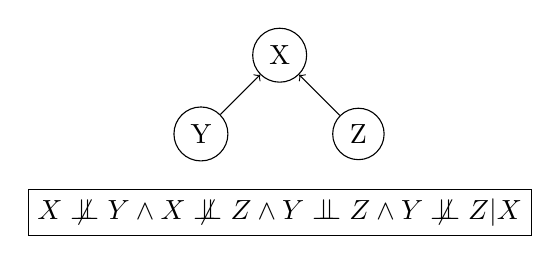
\begin{tikzpicture}
        \path (0,0) node[circle,draw](x) {X} (-1, -1) node[circle,draw](y) {Y} (1, -1) node[circle,draw](z) {Z};
        \draw[->] (y) -- (x);
        \draw[->] (z) -- (x);
        \draw (0, -2) node[draw] {$X\nindep Y \wedge X\nindep Z \wedge Y\indep Z \wedge Y\nindep Z|X$};
    \end{tikzpicture}
\end{figure}

\begin{figure}
    \centering
    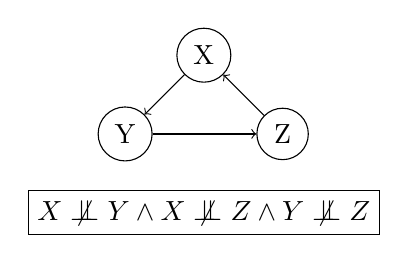
\begin{tikzpicture}
        \path (0,0) node[circle,draw](x) {X} (-1, -1) node[circle,draw](y) {Y} (1, -1) node[circle,draw](z) {Z};
        \draw[->] (x) -- (y);
        \draw[->] (y) -- (z);
        \draw[->] (z) -- (x);
        \draw (0, -2) node[draw] {$X\nindep Y \wedge X\nindep Z \wedge Y\nindep Z$};
    \end{tikzpicture}
    \label{tikz:bay_last}
\end{figure}

\section{}
\subsection{}
We have given \(p(\B{x}) = \N(\B{x}|\B{\μ},\B{\Sigma})\) and \(q(\B{x}) = \N(\B{x}|\B{m},\B{L})\). \(\B{x}\∈\ℝ^k\).

\begin{align*}
    \ln q(\B{x})
    &= -\÷{k}{2}\ln{(2\π)} -\÷{1}{2}|\B{L}| - \÷{1}{2}(\B{x} - \B{m})^T\B{L}^{-1}(\B{x} - \B{m})\\
    \KL(p||q)
    &= -\int p(\B{x}) \ln{(\÷{q(\B{x})}{p(\B{x})})} d\B{x}\\
    &= -\int p(\B{x}) \left[\ln q(\B{x}) - \ln p(\B{x}) \right]d\B{x}\\
    &= \int p(\B{x})\ln p(\B{x}) d\B{x} - \int p(\B{x})\ln q(\B{x})d\B{x}\\
    &= -\mathcal{H}(p(\B{X})) - \int p(\B{x})\ln q(\B{x})d\B{x}\\
    &= -\mathcal{H}(p(\B{X})) +\÷{k}{2}\ln{(2\π)} + \÷{1}{2}|\B{L}| +\÷{1}{2} \int p(\B{x})(\B{x} - \B{m})^T\B{L}^{-1}(\B{x} - \B{m})d\B{x}\\
    &= -\÷{k}{2} -\÷{k}{2}\ln{(2\π)} -\÷{1}{2}\ln |\B{\Sigma}| +\÷{k}{2}\ln{(2\π)} + \÷{1}{2}|\B{L}| +\÷{1}{2} \int p(\B{x})(\B{x} - \B{m})^T\B{L}^{-1}(\B{x} - \B{m})d\B{x}\\
    &= -\÷{k}{2} +\÷{1}{2}\÷{|\B{L}|}{|\B{\Sigma}|} +\÷{1}{2}\int p(\B{x})(\B{x} - \B{m})^T\B{L}^{-1}(\B{x} - \B{m})d\B{x}\\
    &= -\÷{k}{2} +\÷{1}{2}\÷{|\B{L}|}{|\B{\Sigma}|} +\÷{1}{2} \E[(\B{x} - \B{m})^T\B{L}^{-1}(\B{x} - \B{m})]_{p(\B{x})}\\
    &= -\÷{k}{2} +\÷{1}{2}\÷{|\B{L}|}{|\B{\Sigma}|} +\÷{1}{2} [(\B{\μ} - \B{m})^T\B{L}^{-1}(\B{\μ} - \B{m}) + \Tr{(\B{L}^{-1}\B{\Sigma})}]\\
    &= \÷{1}{2} \left[\÷{|\B{L}|}{|\B{\Sigma}|} -k +(\B{\μ} - \B{m})^T\B{L}^{-1}(\B{\μ} - \B{m}) +\Tr{(\B{L}^{-1}\B{\Sigma})}\right]\\
\end{align*}

\subsection{}
\begin{align*}
    \ln p(\B{x})
    &= -\÷{k}{2}\ln{(2\π)} -\÷{1}{2}|\B{\Sigma}| - \÷{1}{2}(\B{x} - \B{\μ})^T\B{\Sigma}^{-1}(\B{x} - \B{\μ})\\
    \mathcal{H}(p)
    &= -\int p(\B{x})\ln p(\B{x})d\B{x}\\
    &= \÷{k}{2}\ln{(2\π)} +\÷{1}{2}|\B{\Sigma}| +\÷{1}{2}\E_{p(\B{x})}\left[(\B{x} - \B{\μ})^T\B{\Sigma}^{-1}(\B{x} - \B{\μ})\right]\\
    &= \÷{k}{2}\ln{(2\π)} +\÷{1}{2}|\B{\Sigma}| +\÷{1}{2}\E_{p(\B{x})}\left[\Tr((\B{x} - \B{\μ})^T\B{\Sigma}^{-1}(\B{x} - \B{\μ}))\right]\\
    &= \÷{k}{2}\ln{(2\π)} +\÷{1}{2}|\B{\Sigma}| +\÷{1}{2}\E_{p(\B{x})}\left[\Tr(\B{\Sigma}^{-1}(\B{x} - \B{\μ})^T(\B{x} - \B{\μ}))\right]\\
    &= \÷{k}{2}\ln{(2\π)} +\÷{1}{2}|\B{\Sigma}| +\÷{1}{2}\Tr\left(\B{\Sigma}^{-1}\E_{p(\B{x})}\left[(\B{x} - \B{\μ})^T(\B{x} - \B{\μ})\right]\right)\\
    &= \÷{k}{2}\ln{(2\π)} +\÷{1}{2}|\B{\Sigma}| +\÷{1}{2}\Tr\left(\B{\Sigma}^{-1}\E_{p(\B{x})}\left[\B{\Sigma}\right]\right)\\
    &= \÷{k}{2}\ln{(2\π)} +\÷{1}{2}|\B{\Sigma}| +\÷{1}{2}\Tr\left(\B{\Sigma}^{-1}\B{\Sigma}\right)\\
    &= \÷{k}{2}\ln{(2\π)} +\÷{1}{2}|\B{\Sigma}| +\÷{1}{2}\Tr\left(\1_k\right)\\
    &= \÷{k}{2}\ln{(2\π)} +\÷{1}{2}|\B{\Sigma}| +\÷{k}{2}\\
\end{align*}

\end{document}
